\documentclass[11pt, a4paper]{article}
\usepackage[utf8]{inputenc}
\usepackage{geometry}
\geometry{a4paper, margin=0.8in}
\usepackage{graphicx}
\usepackage[table]{xcolor}
\usepackage{hyperref}
\usepackage{array}

% Define Colors
\definecolor{cyanHeader}{HTML}{00AEEF}
\definecolor{yellowSub}{HTML}{FFF2CC}
\definecolor{blueBorder}{HTML}{0070C0}
\definecolor{blueBg}{HTML}{E5F0F9}
\definecolor{pinkBg}{HTML}{FCE4D6}
\definecolor{pinkBorder}{HTML}{FF9999}
\definecolor{cyanBg}{HTML}{D9F8FB}
\definecolor{cyanBorder}{HTML}{70DBDB}
\definecolor{greenBg}{HTML}{D9F2E6}
\definecolor{greenBorder}{HTML}{70C090}
\definecolor{orangeBorder}{HTML}{ED7D31}
\definecolor{sectionBlue}{HTML}{4472C4}

% Custom Box Command
\newcommand{\cbox}[3]{
    \noindent\fcolorbox{#1}{#2}{
        \parbox{\dimexpr\textwidth-2\fboxsep-2\fboxrule\relax}{#3}
    }
}

\setlength{\parindent}{0pt}
\setlength{\fboxsep}{8pt}

\begin{document}

% Header Block
\cbox{cyanHeader}{cyanHeader}{
    \centering\bfseries\color{white}\large MSME IDEA HACKATHON 6.0\\Frontier Technology in MSMEs
}
\vspace{0.6cm}

% Title
\begin{center}
    {\large \textbf{FPDAF (Federated Personalized Drift Alerting Framework): CLINICAL AI EARLY-WARNING WORKSTATION}}\\[0.2cm]
    {Explainable Federated Learning for Sepsis CDSS with Personalized Drift Adaptation}\\[0.4cm]
    
    \fcolorbox{black}{yellowSub}{
        \parbox{0.6\textwidth}{\centering \textbf{SUB-THEME 6: OTHER FRONTIER TECHNOLOGIES}}
    }
\end{center}
% Executive Summary
{\Large\color{sectionBlue} EXECUTIVE SUMMARY}
\vspace{0.2cm}

\cbox{blueBorder}{blueBg}{
    \textbf{(i) Summary of Proposed Project Goal:}\\
    We propose to develop and implement \textbf{FPDAF (Federated Personalized Drift Alerting Framework)}, an intelligent, secure Clinical Decision Support System (CDSS) designed to detect sepsis early in intensive care units (ICUs) while preserving patient data privacy through federated learning.\\
    We aim to install local Edge-AI compute nodes at clinical bedside stations to monitor patient vital streams in real-time, providing early clinical alerts while keeping sensitive patient records local to support data privacy compliance.\\[0.2cm]
    The proposed system is designed for deployment across government hospitals, medical colleges, district hospitals, and corporate healthcare networks, supporting India's Ayushman Bharat Digital Mission (ABDM) through secure, privacy-preserving AI-based clinical decision support.\\[0.2cm]
    \textbf{TRL Verification \& Validation Status (TRL 4/5):} The proposed framework's core algorithms are under active development and testing, validated using simulated hospital networks on historical EHR ICU data. The proposed solution has been architected for scalable deployment and pilot validation within Indian public healthcare environments. The backend analytics engine and the clinician dashboard prototype are being prepared for shadow pilot runs. A functional workstation demo has been archived for verification on GitHub.\\[0.2cm]
    \textbf{Clinical Mentorship \& Review:} We are in active communication and collaboration with clinical experts and intensive care doctors to guide the protocol design, clinical review, and non-interventional validation of the proposed system.
}
\vspace{0.4cm}

% Metrics
\noindent
\fcolorbox{pinkBorder}{pinkBg}{\parbox{\dimexpr0.31\textwidth-2\fboxsep-2\fboxrule\relax}{\centering 2.9--3.0M\\Sepsis Deaths/Year in India [1]}}%
\hfill
\fcolorbox{orangeBorder}{yellowSub}{\parbox{\dimexpr0.31\textwidth-2\fboxsep-2\fboxrule\relax}{\centering 8\%/hour\\Survival Decrease if Delayed [2]}}%
\hfill
\fcolorbox{cyanBorder}{cyanBg}{\parbox{\dimexpr0.31\textwidth-2\fboxsep-2\fboxrule\relax}{\centering 34--50\%\\ICU Mortality Rate Range [3]}}
\vspace{0.6cm}

% Sepsis Challenge
{\Large\color{sectionBlue} PROBLEM STATEMENT: THE SEPSIS CHALLENGE}
\vspace{0.2cm}

\textbf{Clinical Problem \& Emotional Narrative:}\\
\textit{Hypothetical Case Study:} Patient Ramesh, 54, is admitted to the ICU with a mild post-operative UTI. Within 6 hours, his vitals silently drift: his breathing accelerates and his oxygen saturation drops marginally. Because no single vital sign is individually "in the red," traditional bedside threshold alarms remain silent. However, a systemic inflammatory response is already cascading. By the time his blood pressure drops, he is in Septic Shock. Resuscitation therapy is now too late, leading to multi-organ failure. Ramesh passes away from a condition that was treatable had it been caught hours earlier.\\[0.2cm]
Every single hour of delayed sepsis treatment increases the risk of mortality by \textbf{8\%} [2]. FPDAF (Federated Personalized Drift Alerting Framework) acts as a clinical early-warning radar system to prevent such catastrophic collapses.

\vspace{0.4cm}
\begin{minipage}{\textwidth}
\textbf{Sepsis Burden \& Impact in India:}

\vspace{0.1cm}
\noindent
\fcolorbox{pinkBorder}{white}{
\parbox{\dimexpr0.48\textwidth-2\fboxsep-2\fboxrule\relax}{
    \textbf{National Mortality \& Case Load}\\
    \textit{\small Sepsis represents a critical public health crisis in India:}\\[0.1cm]
    $\bullet$ \textbf{2.9 to 3.0 Million Deaths:} Estimated annually across India due to Sepsis [1].\\
    $\bullet$ \textbf{11.0 to 11.3 Million Cases:} Recorded annually nationwide.\\
    $\bullet$ \textbf{Proportional Mortality:} Sepsis accounts for roughly \textbf{30\% (3 in 10)} of all deaths in India.\\[0.1cm]
    \textit{\small Source: The George Institute for Global Health, 2020}
}}
\hfill
\fcolorbox{pinkBorder}{white}{
\parbox{\dimexpr0.48\textwidth-2\fboxsep-2\fboxrule\relax}{
    \textbf{Indian ICU Mortality Metrics}\\
    \textit{\small Within clinical critical care environments:}\\[0.15cm]
    $\bullet$ \textbf{34\% to 50\%+ Mortality Rate:} Severe sepsis patients in Indian ICUs face high clinical mortality [3].\\
    $\bullet$ \textbf{Antimicrobial Resistance (AMR):} High AMR rates complicate treatment, making hours-early detection crucial.\\[0.35cm]
    \textit{\small Source: Indian Society of Critical Care Medicine (ISCCM)}
}}
\end{minipage}

\vspace{0.4cm}
% Pointwise Objectives
{\Large\color{sectionBlue} OBJECTIVES OF THE PROPOSED PROJECT}
\vspace{0.2cm}

We propose the following point-wise clinical and technical objectives for the project:
\begin{itemize}
    \item \textbf{Develop a Privacy-Preserving CDSS:} Implement the FPDAF (Federated Personalized Drift Alerting Framework) to train early-warning models across hospital nodes while keeping sensitive patient records local to support data privacy compliance.
    \item \textbf{Mitigate ICU Sepsis Mortality:} Implement localized, real-time predictive alerts to target a reduction of severe sepsis mortality by up to \textbf{25\%} during pilot deployment in partnering hospitals, demonstrating the potential to improve clinical outcomes across large hospital networks.
    \item \textbf{Reduce Critical Healthcare Costs:} Shorten average ICU length of stay by \textbf{2.2 days}, helping to potentially reduce ICU treatment costs and hospitalization duration.
    \item \textbf{Support Localized Model Adaptation:} Incorporate Client-Side Selective Personalization (CSSP) to ensure the CDSS automatically adapts to different ICU demographics and concepts within minutes.
    \item \textbf{Maintain Clinician Trust:} Generate temporal self-attention heatmaps providing explainable insights into which clinical variables and hours drove each risk alert.
\end{itemize}

\vspace{0.4cm}
\begin{minipage}{\textwidth}
% Proposed Solution
{\Large\color{sectionBlue} PROPOSED SOLUTION \& CLINICAL ARCHITECTURE}
\vspace{0.2cm}

\textbf{(ii) System Overview \& Architecture Diagram:}
\begin{center}
    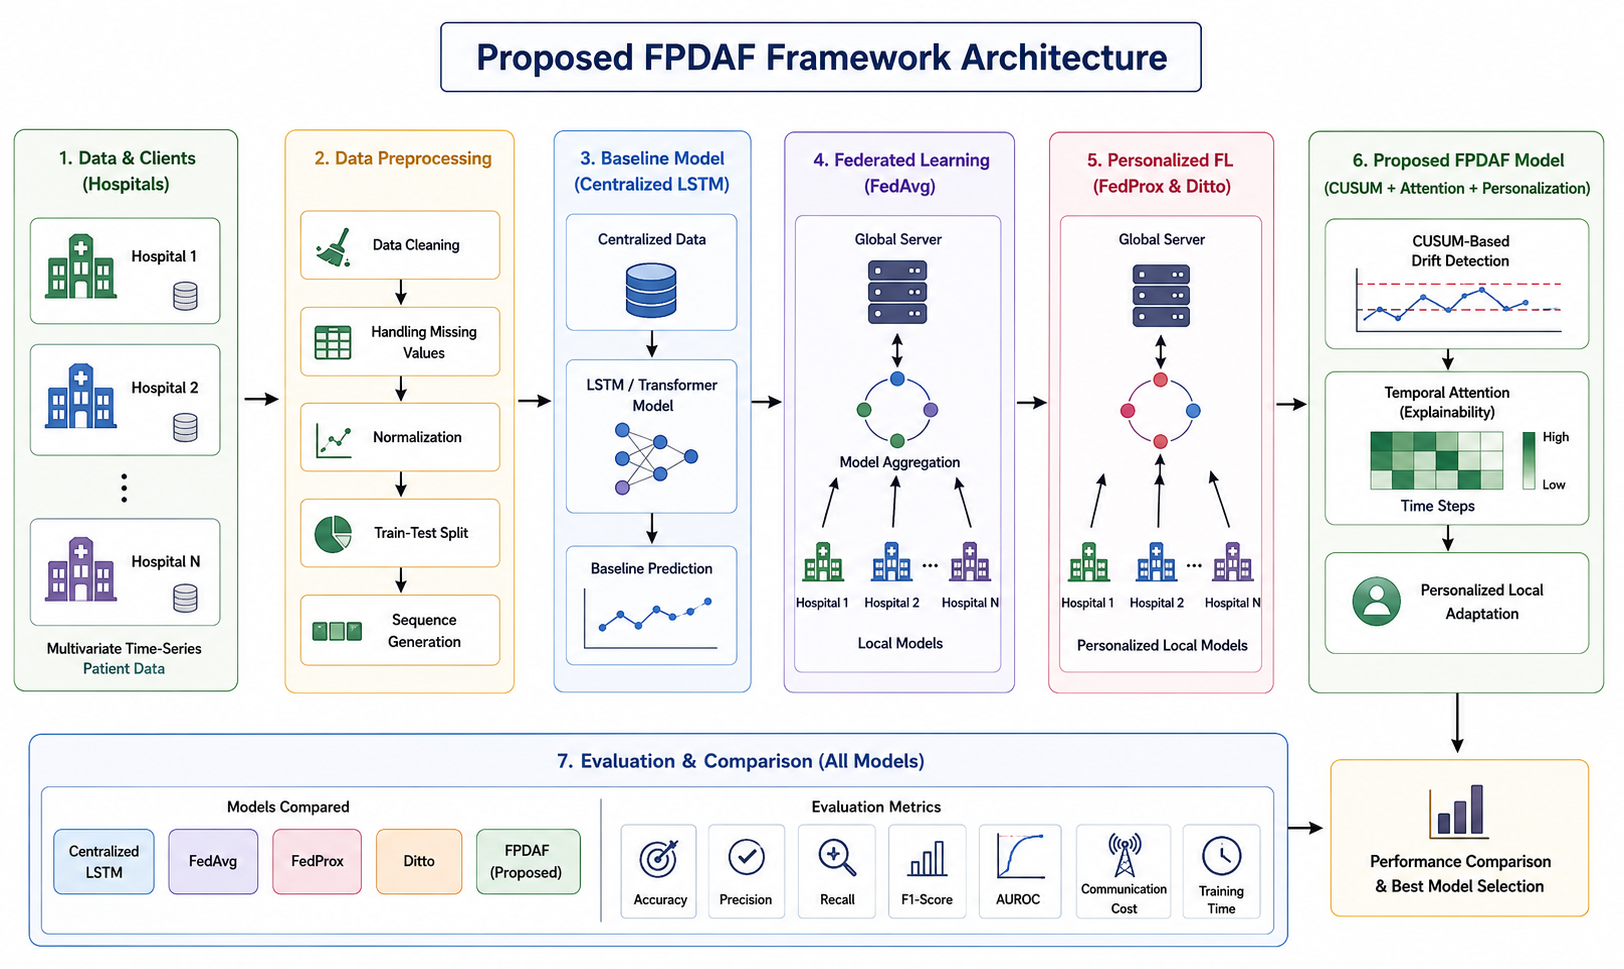
\includegraphics[width=0.82\textwidth]{images/fpdafarcdiagram.png}
\end{center}
\end{minipage}

\textbf{Methodology Description:}\\
The proposed Federated Personalized Drift Alerting Framework (FPDAF) processes local patient vital arrays through a shared Bidirectional Long Short-Term Memory (BiLSTM) neural feature extractor and self-attention query layers. To handle clinical variations across different hospitals, local CUSUM (Cumulative Sum) monitors track data distribution changes to flag concept drifts in real-time. When drift is identified, the Client-Side Selective Personalization (CSSP) protocol is triggered to retrain the local classifier head on local EHR ICU data while keeping the global feature representations secure. This hybrid edge-server architecture enables collaborative model learning without compromising hospital data privacy.


\vspace{0.6cm}

% Technical Innovations & Competitive Analysis
{\Large\color{sectionBlue} INNOVATIVE ANALYSIS \& COMPETITIVE ADVANTAGE}
\vspace{0.2cm}

\textbf{(iii) Key Technical Innovations (Point-wise):}
\begin{itemize}
    \item \textbf{Explainable AI (XAI):} Generates bedside temporal attention heatmaps for clinical validation and user trust.
    \item \textbf{CUSUM Drift Auditing:} Monitors loss residuals to flag patient demographic and concept shifts in real-time.
    \item \textbf{CSSP Calibration:} Saves 38\% network bandwidth and automatically adapts models to new hospital sites in 6 minutes.
    \item \textbf{Government-ready Deployment:} Designed for secure deployment within Indian public healthcare infrastructure while complying with DPDPA and national cybersecurity guidelines.
    \item \textbf{Intellectual Property (IP):} A provisional Indian patent is planned covering the Client-Side Selective Personalization (CSSP) protocol and the CUSUM-based drift adaptation architecture.
\end{itemize}

\vspace{0.2cm}
\textbf{Competitive Matrix: Comparison of Key Capabilities$^*$}\\
\vspace{0.1cm}
\noindent
\fcolorbox{orangeBorder}{white}{
\parbox{\dimexpr\textwidth-2\fboxsep-2\fboxrule\relax}{
\centering
\setlength{\tabcolsep}{3pt}
\renewcommand{\arraystretch}{1.2}
\begin{tabular}{p{3.6cm} c c c c}
\rowcolor{orangeBorder}
\textbf{\textcolor{white}{Feature}} & \textbf{\textcolor{white}{FPDAF (Ours)}} & \textbf{\textcolor{white}{Epic System}} & \textbf{\textcolor{white}{Philips Monitor}} & \textbf{\textcolor{white}{Google Health}} \\
\hline
Federated Privacy & \cellcolor{greenBg}\textbf{Yes} & \cellcolor{pinkBg}No (Cloud) & \cellcolor{pinkBg}No (Local) & \cellcolor{pinkBg}No (Cloud) \\
Concept Drift Auditing & \cellcolor{greenBg}\textbf{Yes} & \cellcolor{pinkBg}No & \cellcolor{pinkBg}No & \cellcolor{pinkBg}No \\
Temporal XAI Heatmaps & \cellcolor{greenBg}\textbf{Yes} & \cellcolor{pinkBg}No & \cellcolor{pinkBg}No & \cellcolor{greenBg}Yes \\
Local Customization (CSSP) & \cellcolor{greenBg}\textbf{Yes} & \cellcolor{pinkBg}No & \cellcolor{pinkBg}No & \cellcolor{pinkBg}No \\
Edge-AI Deployment & \cellcolor{greenBg}\textbf{Yes} & \cellcolor{yellowSub}Partial & \cellcolor{greenBg}Yes & \cellcolor{pinkBg}No \\
DPDPA-Ready Privacy Compliance & \cellcolor{greenBg}\textbf{Yes} & \cellcolor{yellowSub}Partial & \cellcolor{yellowSub}Partial & \cellcolor{yellowSub}Partial \\
\hline
\end{tabular}
}
}
\vspace{0.1cm}
\textit{\small $^*$Based on publicly available product specifications and literature review as of Q2.}\\
\textit{\small $^\dagger$Source: Indian Healthcare CDSS Market Analysis Report (2025).}

\vspace{0.6cm}

% Applications, Market, Business Model
{\Large\color{sectionBlue} MARKET POTENTIAL, BUSINESS MODEL \& RISK ANALYSIS}
\vspace{0.2cm}

\textbf{(iv) Indian MSME Hardware-Software Integration:}
Unlike pure software startups, FPDAF (Federated Personalized Drift Alerting Framework) is proposed as an **integrated medical hardware product**. The product consists of a physical local Edge-AI compute node (the Bedside Workstation box with custom display, visual alarms, and network interface) manufactured and assembled locally in India. This qualifies it as a physical medical technology product suitable for Indian MSME manufacturing scale-up. We have initiated discussions with local embedded electronics MSMEs and medical device manufacturing MSMEs in Coimbatore for PCB assembly and edge hardware enclosure fabrication. This enables a robust local hardware supply chain that aligns directly with MSME manufacturing capabilities.

\textbf{(v) Market Sizing (TAM/SAM/SOM) \& Government Adoption:}\\
Estimated TAM: Rs. 1,000 Crores (India's Clinical Decision Support System market)$^\dagger$.\\
Estimated SAM: Rs. 375 Crores (Corporate/private hospital ICU networks, calculated at Rs. 15,000/bed/year for approx. 2,50,000 private ICU beds).\\
Estimated SOM: Rs. 40 Crores (Regional hospital networks targetable in Years 1--2 representing 12 regional hospital chains).\\
\textbf{Government Adoption Pathways:} The system has high potential for adoption across public healthcare networks. Potential users include AIIMS, State Medical Colleges, Government Hospitals, District Hospitals, Corporate Hospital Chains, and Tele-ICU Networks.\\
\textbf{Commercialization Strategy:} We will scale the system through a 5-Phase strategy: (1) Phase 1: Pilot hospital validation, (2) Phase 2: Regional network deployment, (3) Phase 3: Government procurement and public hospital deployment, (4) Phase 4: Scaling to private hospital networks, and (5) Phase 5: Global export scaling.

\vspace{0.2cm}
\textbf{Revenue Generation Model \& 5-Year Projection:}\\
Monetized via OEM IP Licensing (5\% royalty per device sold by hardware partners), B2B SaaS Subscriptions (Rs. 15,000/bed/year), and Annual Maintenance Contracts (15\% of contract value).\\[0.1cm]
\textbf{Expected Revenue (5-Year Projection):}
\begin{itemize}
    \item \textbf{Year 1:} Rs. 0 (Non-interventional Pilot Phase)
    \item \textbf{Year 2:} Rs. 12,0,000 (Early-adopter private hospital chains)
    \item \textbf{Year 3:} Rs. 45,0,000 (Launch of regional commercial B2B SaaS)
    \item \textbf{Year 4:} Rs. 1,20,0,000 (Scale deployment to Tier-2/3 cities and public sector)
    \item \textbf{Year 5:} Rs. 3,50,0,000 (Global export and deep OEM integrations)
\end{itemize}

\vspace{0.2cm}
\textbf{5-Year Commercialization \& Regulatory Roadmap:}
\begin{itemize}
    \item \textbf{Year 1:} Non-interventional shadow pilot (zero regulatory risk) at 3 partnering regional networks.
    \item \textbf{Year 2:} Secure ISO 13485 certification; file Class B CDSCO Medical Device application. Ensure compliance with the Digital Personal Data Protection Act (DPDPA 2023) and align with Ayushman Bharat Digital Mission (ABDM) interoperability standards.
    \item \textbf{Year 3:} Launch regional commercial B2B SaaS; secure IEC 60601-1-6 approval.
    \item \textbf{Year 4:} Scale to 100+ hospitals across Tier-2/3 cities.
    \item \textbf{Year 5:} Achieve global export readiness and deep OEM integrations.
\end{itemize}

\vspace{0.2cm}
\textbf{Expected Project Deliverables:}\\
\fcolorbox{greenBorder}{greenBg}{
\parbox{\dimexpr\textwidth-2\fboxsep-2\fboxrule\relax}{
    \centering\small
    \vspace{0.1cm}
    \setlength{\tabcolsep}{6pt}
    \renewcommand{\arraystretch}{1.3}
    \begin{tabular}{p{0.45\textwidth} p{0.45\textwidth}}
    $\bullet$ \textbf{Explainable AI CDSS Software} & $\bullet$ \textbf{Edge-AI Bedside Workstation Prototype} \\
    $\bullet$ \textbf{Secure Federated Learning Server} & $\bullet$ \textbf{Clinician Bedside Dashboard} \\
    $\bullet$ \textbf{Hospital Edge-AI Deployment Toolkit} & $\bullet$ \textbf{Regulatory Documentation \& Audit Pack}
    \end{tabular}
    \vspace{0.1cm}
}
}

\vspace{0.4cm}
\textbf{Risk Analysis \& Mitigation:}

\vspace{0.1cm}
\noindent
\fcolorbox{pinkBorder}{white}{
\parbox{\dimexpr\textwidth-2\fboxsep-2\fboxrule\relax}{
\centering
\setlength{\tabcolsep}{4pt}
\renewcommand{\arraystretch}{1.2}
\begin{tabular}{p{3.8cm} c p{7.2cm}}
\rowcolor{pinkBorder}
\textbf{Identified Risk} & \textbf{Impact} & \textbf{Mitigation Strategy} \\
\hline
Clinical Data Drift & High & CUSUM monitor detects drift; CSSP automatically recalibrates. \\
Poor Hospital IT Infra & Medium & We deploy self-contained, pre-calibrated Edge-AI nodes. \\
CDSCO Regulatory Delay & High & Run shadow pilots to gather evidence while waiting for CDSCO. \\
Clinical Adoption Fatigue & Low & Integrate intuitive temporal XAI heatmaps to prevent alert fatigue. \\
Telemetry Missing Values & Medium & Preprocess pipeline incorporates forward-filling and imputation. \\
Cybersecurity Attacks & High & End-to-end encryption, role-based access, and secure federated aggregation. \\
\hline
\end{tabular}
}
}

\vspace{0.6cm}

\begin{minipage}{\textwidth}
% Budget
{\Large\color{sectionBlue} PROJECT BUDGET REQUIREMENTS}
\vspace{0.2cm}

\cbox{blueBorder}{blueBg}{
    \textbf{(vi) Total Requested Funding: Rs. 15,0,000 (MSME Hackathon Maximum Cap)}\\[0.3cm]
    \noindent
    \centering
    \setlength{\tabcolsep}{6pt}
    \renewcommand{\arraystretch}{1.3}
    \begin{tabular}{p{3.8cm} r p{6.8cm}}
    \hline
    \rowcolor{blueBorder}
    \textbf{\textcolor{white}{Budget Category}} & \textbf{\textcolor{white}{Amount (Rs.)}} & \textbf{\textcolor{white}{Justified Outlay \& Expected Deliverable}} \\
    \hline
    \textbf{vii) Technology Costs} & 10,0,000 & Prototyping component fabrication, edge hardware prototyping and validation, and embedded assembly (3.6L), Local Clinical Curation/Annotation (3.4L), Penetration testing \& DPDPA compliance audits (3.0L) \\
    \hline
    \textbf{viii) Mentor Charges} & 3,00,000 & Incubation facility support, expert CDSS clinical validation guidance, and regulatory filing mentorship \\
    \hline
    \textbf{ix) Travel Expenses} & 2,00,000 & Travel expenses for physical node setup and clinical data audits across partnering regional ICUs \\
    \hline
    \end{tabular}
}
\end{minipage}

\vspace{0.6cm}

% Conclusion
{\Large\color{sectionBlue} CONCLUSION}
\vspace{0.2cm}

We propose FPDAF (Federated Personalized Drift Alerting Framework) as a vital clinical early-warning CDSS to address the critical Sepsis challenge in Indian ICUs. By integrating federated learning with real-time CUSUM drift auditing and client-side selective personalization, the system enables hospitals to train highly accurate predictive models collaboratively while maintaining privacy-preserving learning compliant with DPDPA principles. Supported by active clinical mentorship, local hardware integration, and a clear regulatory roadmap, the proposed solution stands as a highly viable, high-impact medical technology project.

\vspace{0.2cm}
FPDAF combines Explainable AI, Federated Learning, Edge Computing, and privacy-preserving intelligence into a deployment-ready Clinical Decision Support System capable of supporting India's next-generation digital healthcare ecosystem. The proposed platform is designed for scalable adoption across public and private hospitals while encouraging indigenous AI-enabled medical device manufacturing through Indian MSMEs.

\vspace{0.6cm}

% References
{\Large\color{sectionBlue} REFERENCES}
\vspace{0.2cm}

\small
1. The George Institute for Global Health, "Sepsis in India: Prevalence and Impact Report," New Delhi, India, 2020. Available: \href{https://www.georgeinstitute.org.in/projects/sepsis-in-india-prevalence-study-sips}{\textcolor{blueBorder}{George Institute Project Link}}\\
2. Kumar, A., et al., "Duration of hypotension before initiation of effective antimicrobial therapy is the critical determinant of survival in human septic shock," \textit{Critical Care Medicine}, vol. 34, no. 6, pp. 1589--1596, 2006. Available: \href{https://pubmed.ncbi.nlm.nih.gov/16625125/}{\textcolor{blueBorder}{PubMed ID: 16625125}}\\
3. Indian Society of Critical Care Medicine (ISCCM), "Epidemiology of Sepsis in Indian Intensive Care Units: A Multi-Center Study," \textit{Indian Journal of Critical Care Medicine}, 2019. Available: \href{https://pubmed.ncbi.nlm.nih.gov/30704986/}{\textcolor{blueBorder}{PubMed ID: 30704986}}\\
4. World Health Organization, "Global report on the epidemiology and burden of sepsis: current evidence, identifying gaps and future directions," Geneva, 2020. Available: \href{https://www.who.int/publications/i/item/9789240010789}{\textcolor{blueBorder}{WHO Sepsis Report}}\\
5. Ministry of Law and Justice, Govt. of India, "The Digital Personal Data Protection Act, 2023," \textit{The Gazette of India}, 2023. Available: \href{https://www.meity.gov.in/content/digital-personal-data-protection-act-2023}{\textcolor{blueBorder}{DPDPA 2023 Gazette}}\\
6. McMahan, B., et al., "Communication-Efficient Learning of Deep Networks from Decentralized Data," \textit{Proceedings of AISTATS}, 2017. Available: \href{https://arxiv.org/abs/1602.05629}{\textcolor{blueBorder}{arXiv:1602.05629}}\\
7. Vaswani, A., et al., "Attention is all you need," \textit{Advances in Neural Information Processing Systems (NeurIPS)}, 2017. Available: \href{https://arxiv.org/abs/1706.03762}{\textcolor{blueBorder}{arXiv:1706.03762}}\\
8. National Health Authority (NHA), Govt. of India, "Ayushman Bharat Digital Mission (ABDM) Interoperability Guidelines," 2024. Available: \href{https://abdm.gov.in/}{\textcolor{blueBorder}{ABDM Interoperability Link}}

\end{document}
